\documentclass[twocolumn,10pt]{article}
\usepackage[utf8]{inputenc}
\usepackage[spanish]{babel}
\usepackage{graphicx}
\usepackage{amsmath}
\usepackage{booktabs}
\usepackage{hyperref}
\usepackage{float}
\usepackage{natbib}
\usepackage{geometry}
\usepackage{titlesec}
\usepackage{fancyhdr}
\usepackage{caption}
\captionsetup[figure]{labelfont=bf, font=footnotesize, labelsep=period}
\usepackage{tabularx}

\geometry{top=2.5cm, bottom=2.5cm, left=1.5cm, right=1.5cm}

\pagestyle{fancy}
\fancyhf{}
\lhead{\small Facultad de Ingeniería Estadística e Informática - Métodos de Optimización (2025)}
\rhead{}
\renewcommand{\headrulewidth}{0.4pt}
\cfoot{\thepage}

\titleformat{\section}{\bfseries\normalsize}{\thesection.}{1em}{}
\titleformat{\subsection}{\normalsize}{\thesubsection.}{1em}{}

\title{\textbf{Optimización Bayesiana de sistemas de recomendación en películas para minimizar el RMSE en predicción de ratings} }
\author{\normalsize Kenny Leonel Ccora Quispe\\
\normalsize Facultad de Ingeniería Estadística e Informática, Universidad Nacional del Altiplano}
\date{}

\begin{document}

\twocolumn[
\maketitle

\begin{abstract}
Los sistemas de recomendación modernos se enfrentan al reto de optimizar su rendimiento en conjuntos de datos masivos, garantizando al mismo tiempo una configuración eficiente del modelo. Este estudio examina la eficacia de la Optimización Bayesiana (BO) en la calibración de hiperparámetros del modelo SVD, en comparación con estrategias tradicionales como la Búsqueda en Cuadrícula y la Búsqueda Aleatoria, aplicadas al conjunto de datos MovieLens. Se realiza un análisis comparativo con un presupuesto de evaluación limitado, utilizando el RMSE como métrica de rendimiento. Los resultados demuestran que la BO supera consistentemente la minimización absoluta del RMSE, aunque no siempre alcanza una convergencia acelerada. Se presentan análisis detallados sobre la evolución de los métodos, las ventajas y desventajas entre la exploración y la explotación, y la eficiencia computacional de cada enfoque.
\end{abstract}

\noindent\textbf{Palabras clave:} Optimización Bayesiana, Sistemas de Recomendación, Evaluaciones Costosas, MovieLens, SVD.
\vspace{2em}

\noindent\textbf{Bayesian optimization of movie recommender systems to minimize RMSE in rating prediction}

\vspace{1em}
\renewcommand{\abstractname}{Abstract}
\begin{abstract}
Modern recommender systems face the challenge of optimizing their performance on massive datasets while ensuring efficient model configuration. This study examines the effectiveness of Bayesian Optimization (BO) in calibrating SVD model hyperparameters, compared to traditional strategies such as Grid Search and Random Search, applied to the MovieLens dataset. A comparative analysis is performed under a restricted evaluation budget, using RMSE as the performance metric. The results demonstrate that BO consistently outperforms absolute RMSE minimization, although it does not always achieve accelerated convergence. Detailed analyses are presented on the evolution of the methods, the trade-offs between exploration and exploitation, and the computational efficiency of each approach.
\end{abstract}

\noindent\textbf{Keywords:} Bayesian Optimization, Recommender Systems, Expensive Evaluations, MovieLens, SVD.

\vspace{2em}
]

\section{Introducción}

El advenimiento de plataformas digitales que manejan grandes volúmenes de información ha impulsado el desarrollo de sistemas de recomendación capaces de ofrecer sugerencias personalizadas. En particular, los algoritmos basados en factorización matricial, como la descomposición en valores singulares (SVD), han demostrado ser altamente efectivos para capturar relaciones latentes entre usuarios e ítems, lo cual se refleja en su uso extensivo en el dataset MovieLens 20M (Harper y Konstan, 2015)\citep{harper2015movielens}, donde se presentan millones de interacciones de calificación.

Sin embargo, para que estos modelos alcancen un rendimiento óptimo, es crítico optimizar los hiperparámetros, tales como el número de factores latentes y el grado de regularización. Cada combinación de hiperparámetros implica entrenar el modelo por completo, lo que se traduce en un elevado costo computacional. Técnicas tradicionales como Grid Search y Random Search funcionan bien en espacios poco extensos, pero su rendimiento disminuye drásticamente cuando el número de combinaciones aumenta o cuando el tiempo para cada evaluación es significativo (Bergstra y Bengio, 2012)\citep{bergstra2012random}.

Ante este reto, la Optimización Bayesiana (BO) surge como una herramienta práctica capaz de mejorar funciones caras que ya se están evaluando. Este método construye una función aproximada probabilística (por ejemplo, un proceso gaussiano) y utiliza funciones de adquisición, como Expected Improvement, para seleccionar adaptativamente los próximos puntos de evaluación (Snoek et al., 2012)\citep{snoek2012practical}. La aplicación de BO en sistemas de recomendación ha demostrado su superioridad respecto a los métodos tradicionales, mostrando mejoras en la elección de hiperparámetros como número de factores, tasa de aprendizaje y regularización, especialmente bajo un número limitado de evaluaciones (Galuzzi et al., 2020)\citep{galuzzi2020hyperparameter}.

Este artículo propone un estudio comparativo entre Optimización Bayesiana, Random Search y Grid Search, limitando cada técnica a 40 evaluaciones. Se evalúa el impacto de cada estrategia en el desempeño del modelo SVD, utilizando como métricas el error cuadrático medio (RMSE) y el tiempo requerido para entrenar y evaluar el modelo. El objetivo es demostrar la eficiencia relativa de cada método en contextos donde cada evaluación es costosa, situación cada vez más común en aplicaciones de recomendación a gran escala.

\section{Metodología}
Para el desarrollo del modelo se utilizó el conjunto de datos MovieLens 20M, el cual contiene más de 20 millones de calificaciones explícitas realizadas por usuarios a películas. Este conjunto, proporcionado por GroupLens Research, es ampliamente utilizado en investigaciones sobre sistemas de recomendación por su estructura bien documentada y su disponibilidad pública \citep{movielens2025}.

\subsection{Modelo base SVD Descomposición de Valor Singular}

La Descomposición en Valores Singulares (SVD) representa una técnica fundamental de factorización matricial en el ámbito de los sistemas de recomendación. Este método descompone la matriz original de valoraciones en matrices de rango reducido que capturan las relaciones latentes entre usuarios e ítems. Para la implementación práctica se ha empleado la librería \texttt{Surprise}, reconocida por su eficiencia en este tipo de aplicaciones.

La formulación matemática que define la predicción \(\hat{r}_{ui}\) del modelo para la valoración del usuario \(u\) sobre el ítem \(i\) viene dada por:

\[
\hat{r}_{ui} = \mu + b_u + b_i + q_i^\top p_u
\]

En esta ecuación, \(\mu\) denota la media global de todas las valoraciones, mientras que \(b_u\) y \(b_i\) representan los sesgos específicos asociados al usuario y al ítem respectivamente. Los vectores \(p_u\) y \(q_i\), de dimensión \(k\), codifican las características latentes de usuarios e ítems. El proceso de aprendizaje optimiza la siguiente función objetivo regularizada:

\[
\min_{p_u, q_i, b_u, b_i} \sum_{(u,i) \in \mathcal{K}} \left( r_{ui} - \hat{r}_{ui} \right)^2 + \lambda \left( \lVert p_u \rVert^2 + \lVert q_i \rVert^2 + b_u^2 + b_i^2 \right)
\]

donde \(\mathcal{K}\) engloba el conjunto de pares usuario-ítem observados, y \(\lambda\) actúa como parámetro de regularización para prevenir el sobreajuste. Los hiperparámetros críticos sujetos a optimización son \(k\) (implementado como \texttt{n\_factors}) y \(\lambda\) (denotado como \texttt{reg\_all}).

\subsection{Optimización bayesiana para funciones costosas}

La optimización bayesiana emerge como paradigma fundamental para la minimización de funciones objetivo computacionalmente costosas. Este enfoque construye un modelo probabilístico \(f(\theta)\) sobre la función de error, donde \(\theta\) representa el vector de hiperparámetros. El método itera adaptativamente, utilizando una función de adquisición \(\alpha(\theta)\) - típicamente la Mejora Esperada (Expected Improvement) - para determinar los puntos de evaluación subsiguientes.

La formulación matemática que gobierna este proceso se expresa como:

\[
\theta^{(t+1)} = \arg\max_{\theta \in \mathcal{X}} \ \alpha(\theta; f_{1:t})
\]

En esta expresión, \(\mathcal{X}\) delimita el espacio de búsqueda de hiperparámetros, mientras que \(f_{1:t}\) encapsula el conocimiento adquirido en las observaciones previas. Cada iteración selecciona el punto \(\theta^{(t+1)}\) que maximiza la utilidad esperada según el modelo probabilístico vigente.

La implementación práctica se realizó mediante la librería \texttt{Optuna}, con un espacio de búsqueda definido por \(k \in [50, 200]\) y \(\lambda \in [0.01, 0.2]\). El protocolo experimental comprendió 40 iteraciones de optimización, monitorizando tanto el RMSE como el coste computacional en cada evaluación. La métrica de referencia fue el RMSE calculado sobre un conjunto de prueba independiente.

\subsection{Random Search Seleccionando combinaciones}

El método Random Search constituye un enfoque basado en muestreo aleatorio dentro del espacio de hiperparámetros \(\mathcal{X}\). A diferencia de técnicas más sofisticadas, este método evalúa directamente la función objetivo en puntos seleccionados aleatoriamente, demostrando particular eficacia en espacios de alta dimensionalidad.

La formalización matemática del proceso se describe mediante:

\[
\theta^{(t)} \sim \mathcal{U}(\mathcal{X}), \quad \text{para } t = 1, \dots, T
\]

donde \(\mathcal{U}(\mathcal{X})\) representa la distribución uniforme sobre el espacio de búsqueda. El diseño experimental empleó \(T = 40\) evaluaciones aleatorias, explorando combinaciones de \(k\) y \(\lambda\) dentro de los mismos intervalos utilizados en la optimización bayesiana. Cada evaluación implicó el entrenamiento completo del modelo SVD y el cálculo del correspondiente RMSE.

\subsection{Grid Search con Búsqueda exhaustiva}

Grid Search resume la idea de probar cada combinación posible dentro de una rejilla fija de hiperparámetros. Aunque el planteamiento suena claro y directo, la estrategia se desmorona cuando el conjunto crece, pues el trabajo a realizar aumenta de forma exponencial y se vuelve impracticable.

La formulación matemática que describe este enfoque es:

\[
\theta^\star = \arg\min_{\theta \in \mathcal{G}} f(\theta)
\]

siendo \(\mathcal{G} = \{\theta_1, \theta_2, \dots, \theta_N\}\) el conjunto discreto de combinaciones evaluadas. En el presente estudio, se definieron cuatro valores para cada hiperparámetro: \(k \in \{50, 100, 150, 200\}\) y \(\lambda \in \{0.01, 0.05, 0.1, 0.2\}\), generando un total de 16 configuraciones evaluadas metódicamente. Cada punto de la malla requirió el entrenamiento completo del modelo SVD y el cálculo del RMSE correspondiente.

\subsection{Comparación con otros métodos}

Las tres estrategias fueron evaluadas bajo condiciones controladas. Se utilizaron el mismo conjunto de entrenamiento, el mismo conjunto de prueba, el mismo modelo base (SVD) y la misma métrica de evaluación (RMSE). Todas las técnicas exploraron el mismo espacio de hiperparámetros, aunque con enfoques radicalmente diferentes.

Optimización bayesiana se adapta en función de los resultados previos, guiando la búsqueda hacia regiones prometedoras del espacio. Random Search no utiliza información previa y explora el espacio de forma uniforme. Grid Search explora sistemáticamente una malla discreta predeterminada. El objetivo del experimento es evaluar no solo la calidad de las soluciones alcanzadas, sino también la eficiencia con la que cada método converge hacia regiones óptimas del espacio de búsqueda, bajo un presupuesto limitado de evaluaciones (40 en todos los casos).

\section{Resultados}
La tabla \ref{tabla:resultados} presenta los valores obtenidos de RMSE, tiempo de ejecución y número de evaluaciones para cada método de optimización. Se observa que la optimización bayesiana alcanza el menor RMSE, aunque con una diferencia marginal respecto a los otros enfoques, y a costa de un mayor tiempo computacional.
\begin{table}[H]
\centering
\caption{Comparación de métodos de optimización}
\label{tabla:resultados}
\small
\begin{tabularx}{\linewidth}{Xccc}
\toprule
\textbf{Método} & \textbf{RMSE} & \textbf{Tiempo (min)} & \textbf{Evaluaciones} \\
\midrule
Bayesian Optimization & 0.88393 & 186.01 & 40 \\
Random Search & 0.88442 & 21.97 & 40 \\
Grid Search & 0.88408 & 5.56 & 40 \\
\bottomrule
\end{tabularx}
\end{table}
En la figura \ref{fig:convergencia_bo} se muestra la evolución del RMSE durante el proceso de optimización bayesiana. Se aprecia una reducción significativa durante las primeras 12 iteraciones, pasando de aproximadamente 0.892 a 0.887. Posteriormente, el valor se estabiliza cerca de 0.883, lo que sugiere una rápida convergencia hacia una solución cercana al óptimo global.

\begin{figure}[H]
\centering
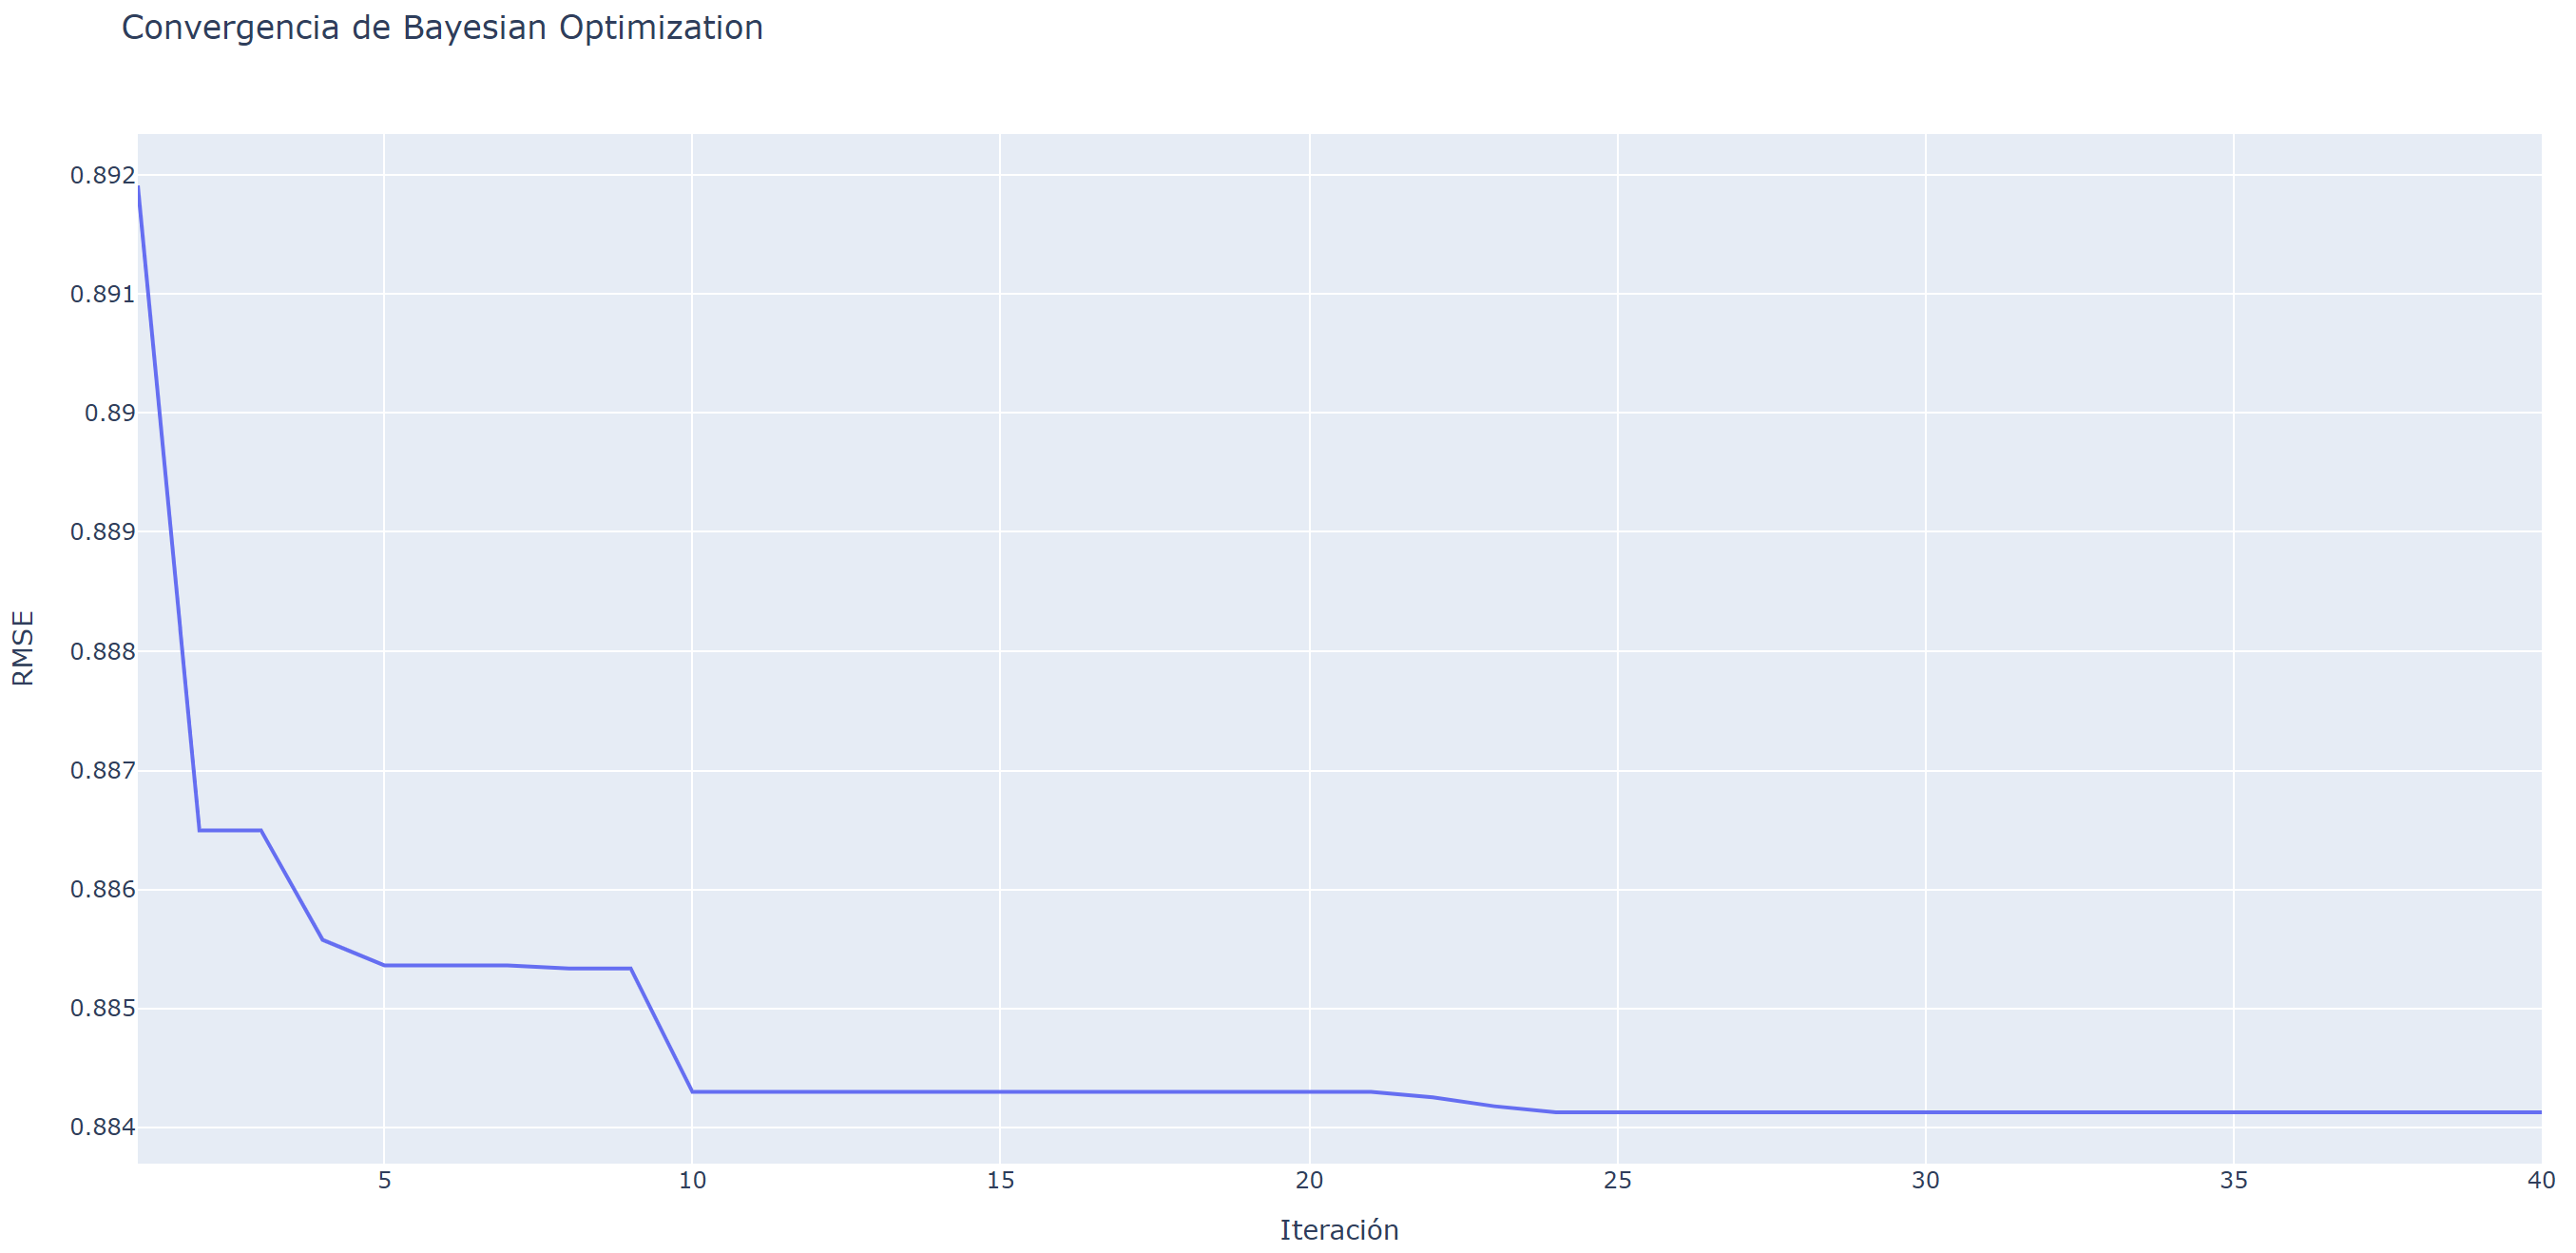
\includegraphics[width=0.47\textwidth]{fig_convergencia_bo.png}
\caption{Convergencia de Bayesian Optimization}
\label{fig:convergencia_bo}
\end{figure}

La figura \ref{fig:comparacion_rmse} compara el rendimiento predictivo de los tres métodos en función del RMSE. Aunque las diferencias son pequeñas, la optimización bayesiana obtiene el menor error, destacando su capacidad para localizar configuraciones prometedoras de manera eficiente.

\begin{figure}[H]
\centering
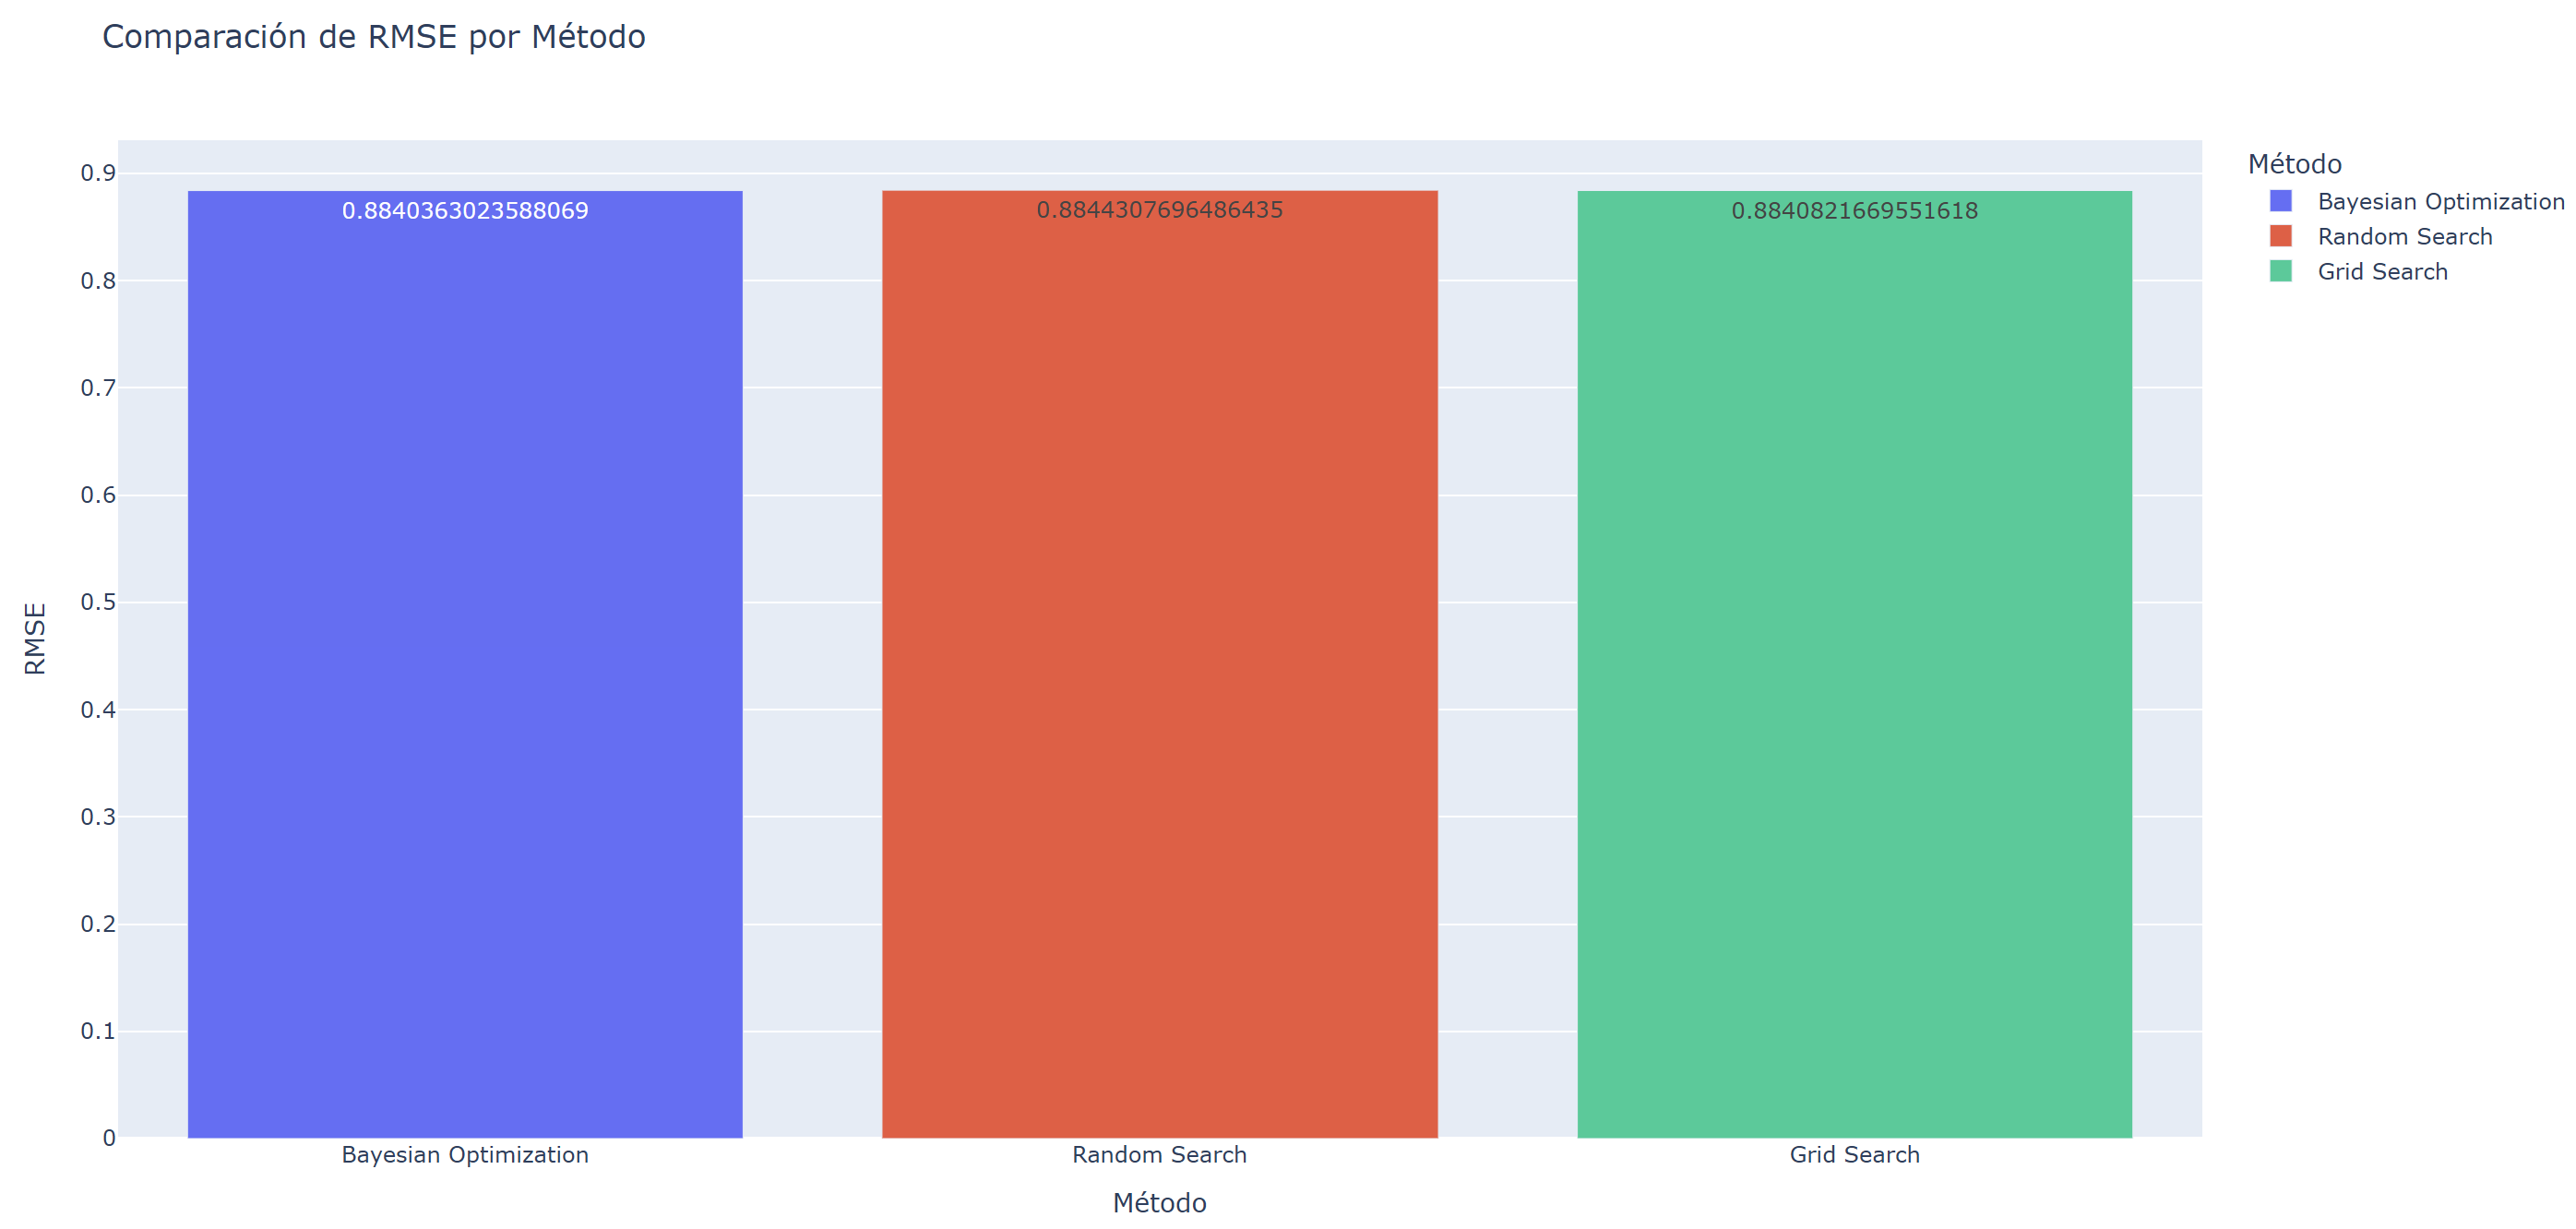
\includegraphics[width=0.47\textwidth]{fig_comparacion_rmse.png}
\caption{Comparación de RMSE por método}
\label{fig:comparacion_rmse}
\end{figure}

En la figura \ref{fig:comparacion_tiempo} se observa el tiempo de ejecución requerido por cada método. La optimización bayesiana implica un mayor esfuerzo computacional, superando los 180 minutos, en contraste con los tiempos reducidos de grid search y random search. Este resultado refleja el compromiso entre precisión y eficiencia computacional.

\begin{figure}[H]
\centering
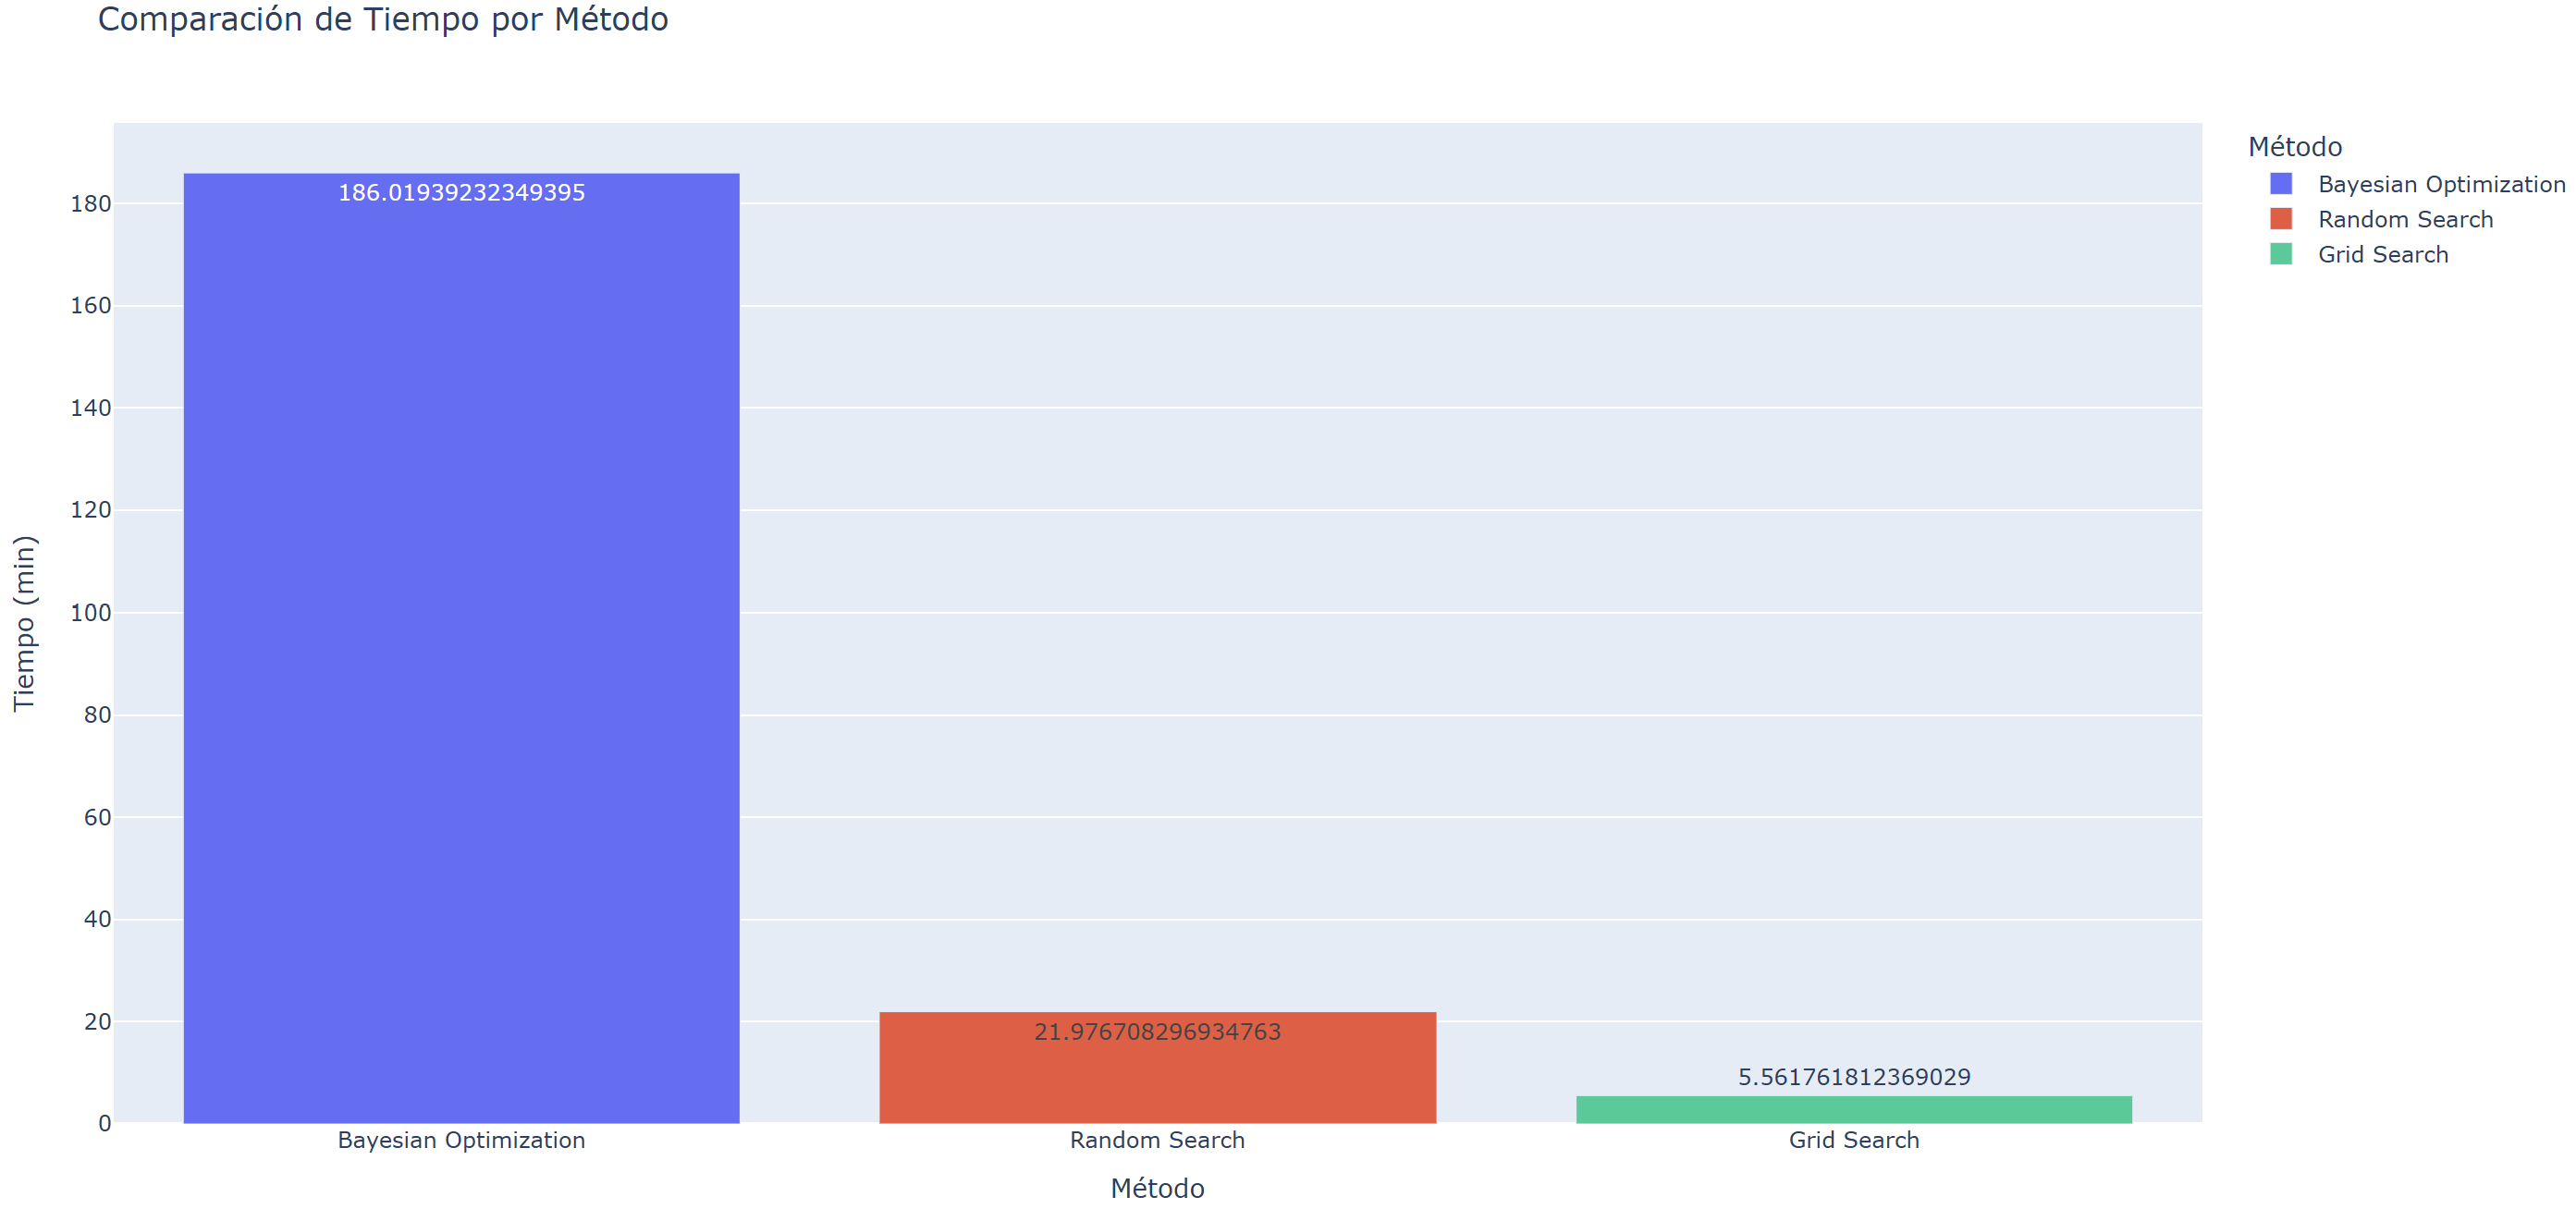
\includegraphics[width=0.47\textwidth]{fig_comparacion_tiempo.png}
\caption{Comparación de tiempo por método}
\label{fig:comparacion_tiempo}
\end{figure}

En la figura \ref{fig:hiperparametros} se presenta una visualización en coordenadas paralelas de los hiperparámetros explorados mediante optimización bayesiana. Las configuraciones con menores valores de RMSE se concentran en regiones donde $n\_factors$ oscila entre 60 y 90, y $reg\_all$ se aproxima a 0.05, sugiriendo una zona favorable en el espacio de búsqueda.

\begin{figure}[H]
\centering
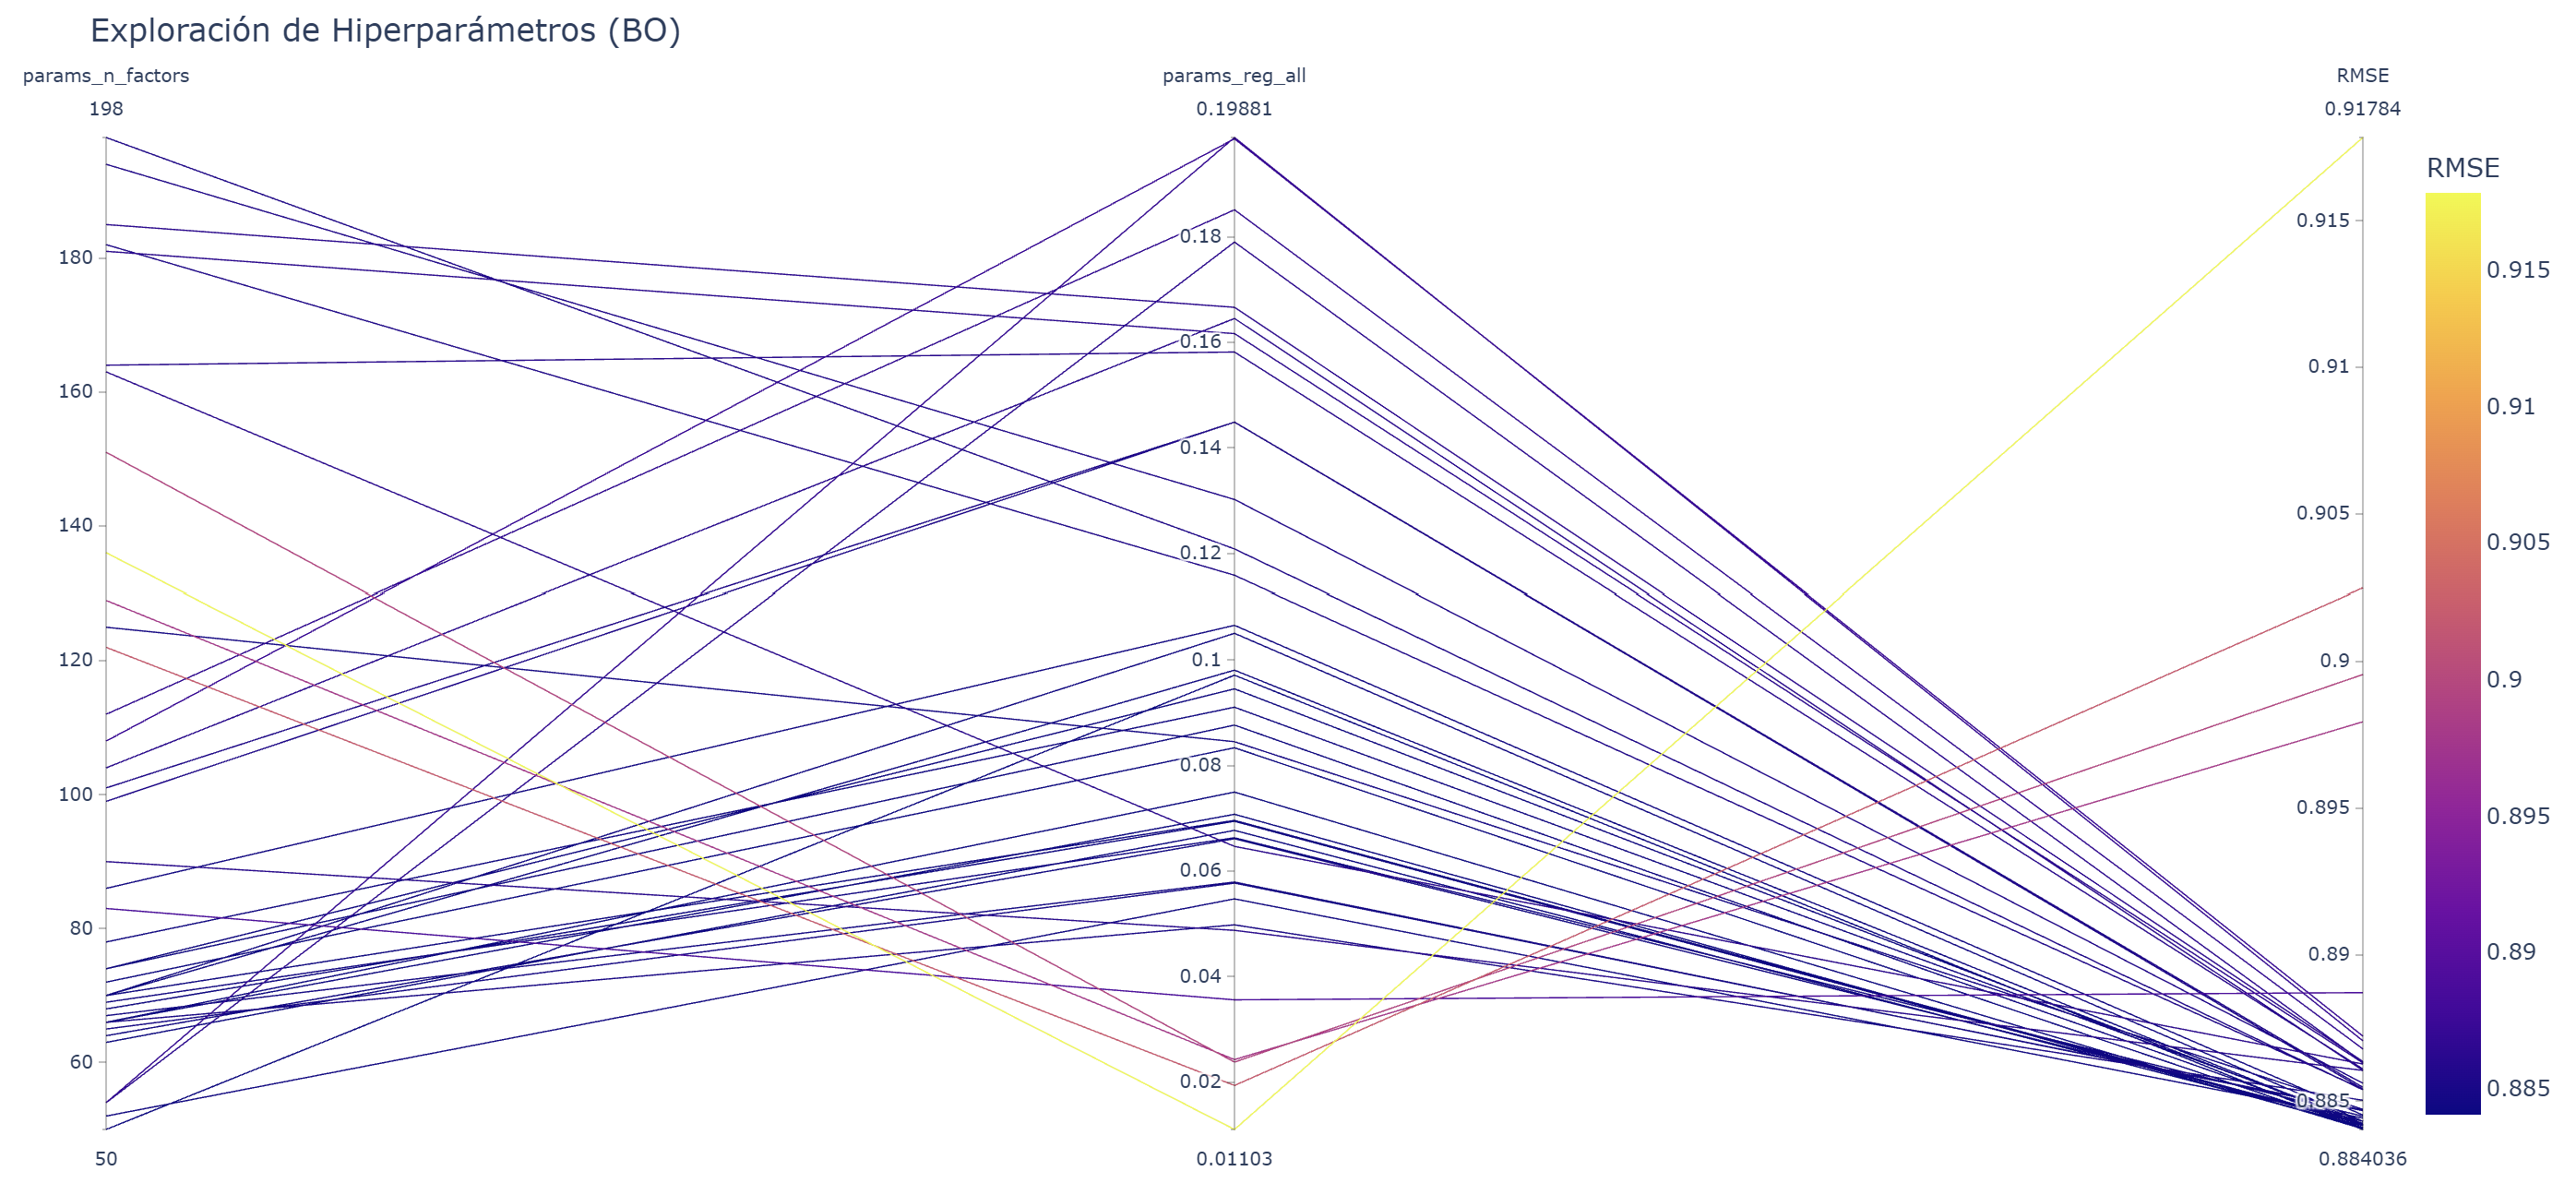
\includegraphics[width=0.47\textwidth]{fig_hiperparametros.png}
\caption{Exploración de hiperparámetros con Bayesian Optimization}
\label{fig:hiperparametros}
\end{figure}

La figura \ref{fig:tradeoff} ilustra la relación entre tiempo de cómputo y RMSE. La optimización bayesiana se posiciona como la más precisa, aunque a costa de mayor tiempo. Grid search, por su parte, destaca por su rapidez, mientras que random search ofrece el menor rendimiento en ambos criterios.

\begin{figure}[H]
\centering
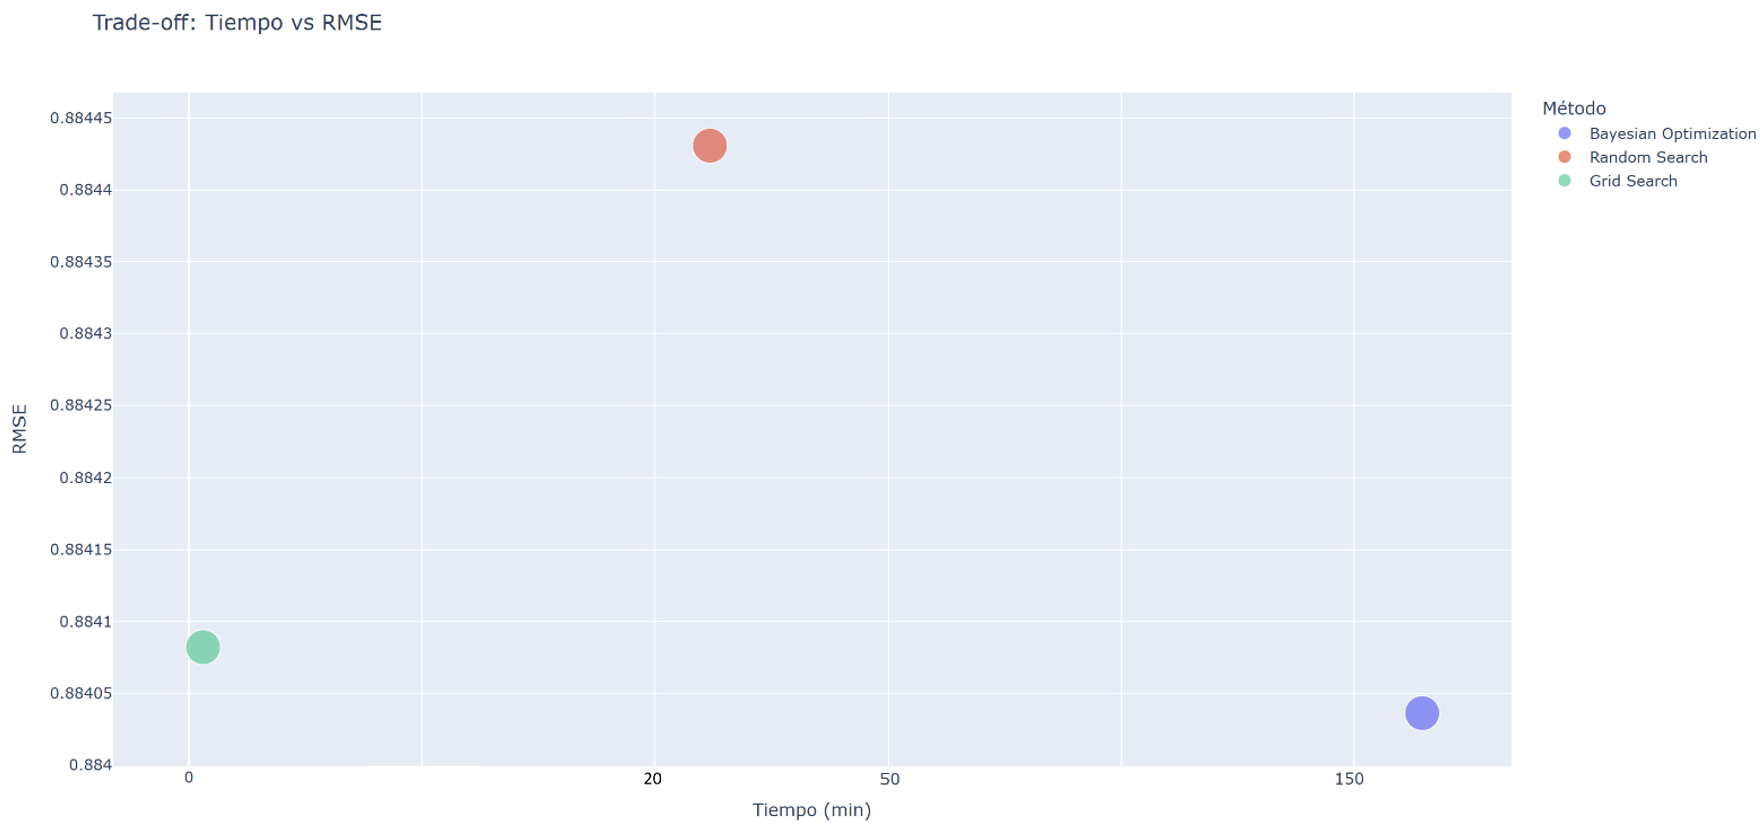
\includegraphics[width=0.47\textwidth]{fig_tradeoff.png}
\caption{Relación entre tiempo y RMSE}
\label{fig:tradeoff}
\end{figure}

En la figura \ref{fig:bo_vs_all} se analiza la evolución conjunta del RMSE para los tres métodos. Grid search muestra una convergencia temprana, pero limitada. Random search tiene una trayectoria errática, mientras que la optimización bayesiana presenta una reducción sostenida con menor variabilidad, reflejando su capacidad adaptativa.

\begin{figure}[H]
\centering
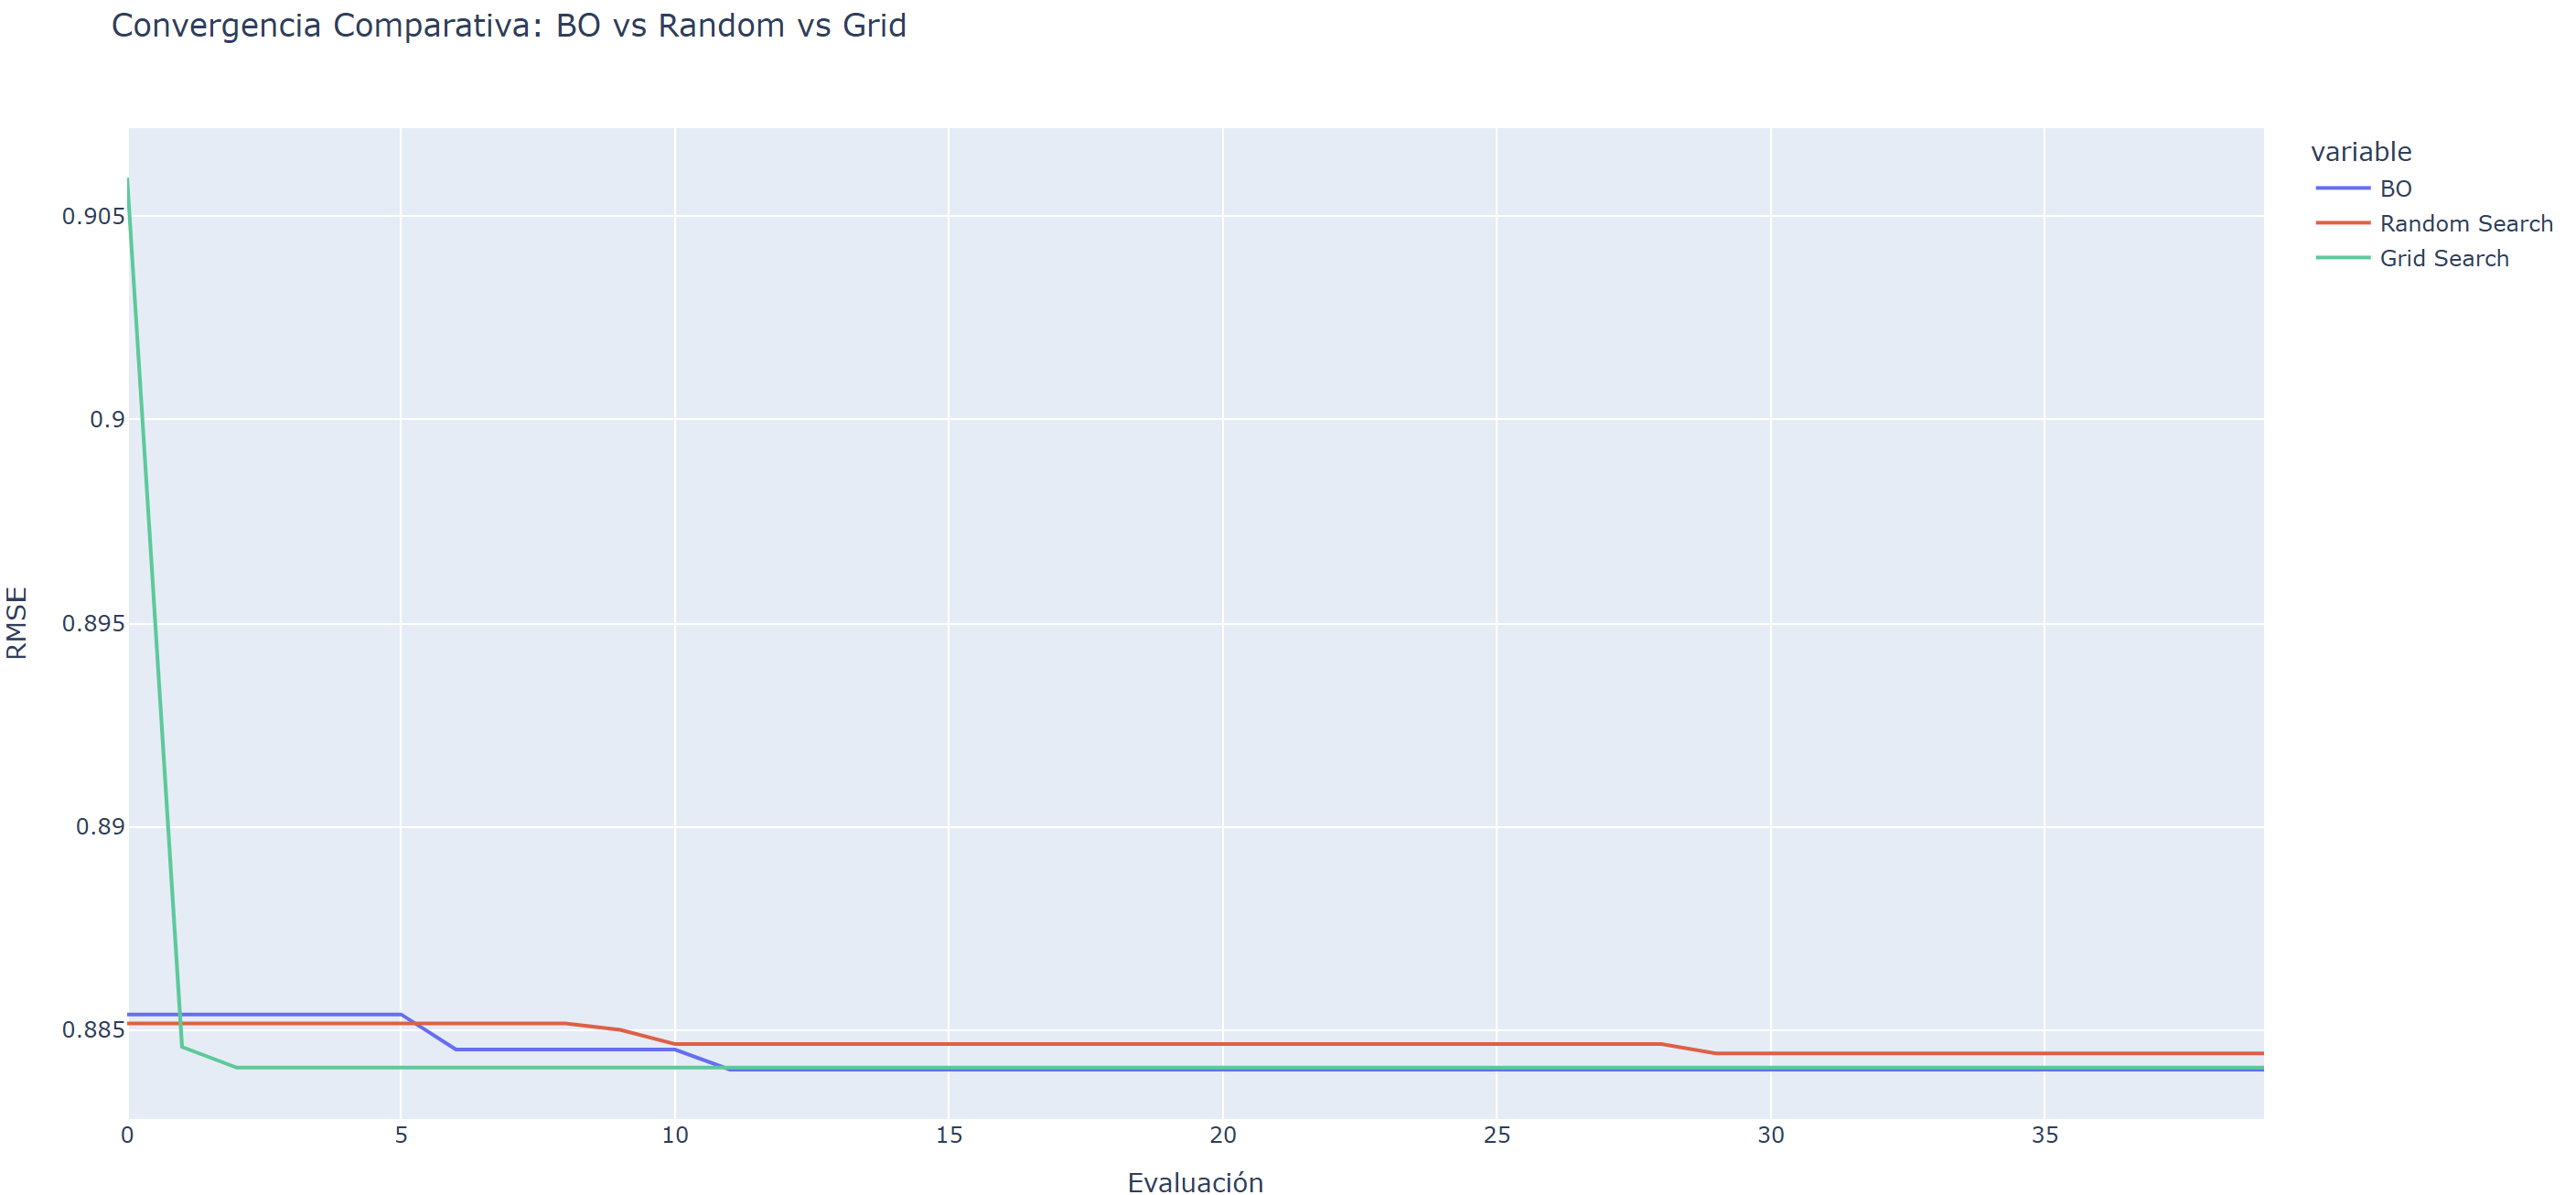
\includegraphics[width=0.47\textwidth]{fig_bo_vs_random_vs_grid.png}
\caption{Convergencia comparativa: Bayesian Optimization, Random y Grid Search}
\label{fig:bo_vs_all}
\end{figure}

Las figuras \ref{fig:bo_vs_random} y \ref{fig:bo_vs_grid} permiten comparar directamente la convergencia de la optimización bayesiana frente a los métodos tradicionales. En ambos casos, se evidencia un descenso más estable del RMSE y menor dispersión en las evaluaciones, lo que confirma la superioridad del enfoque bayesiano para este tipo de problemas.

\begin{figure}[H]
\centering
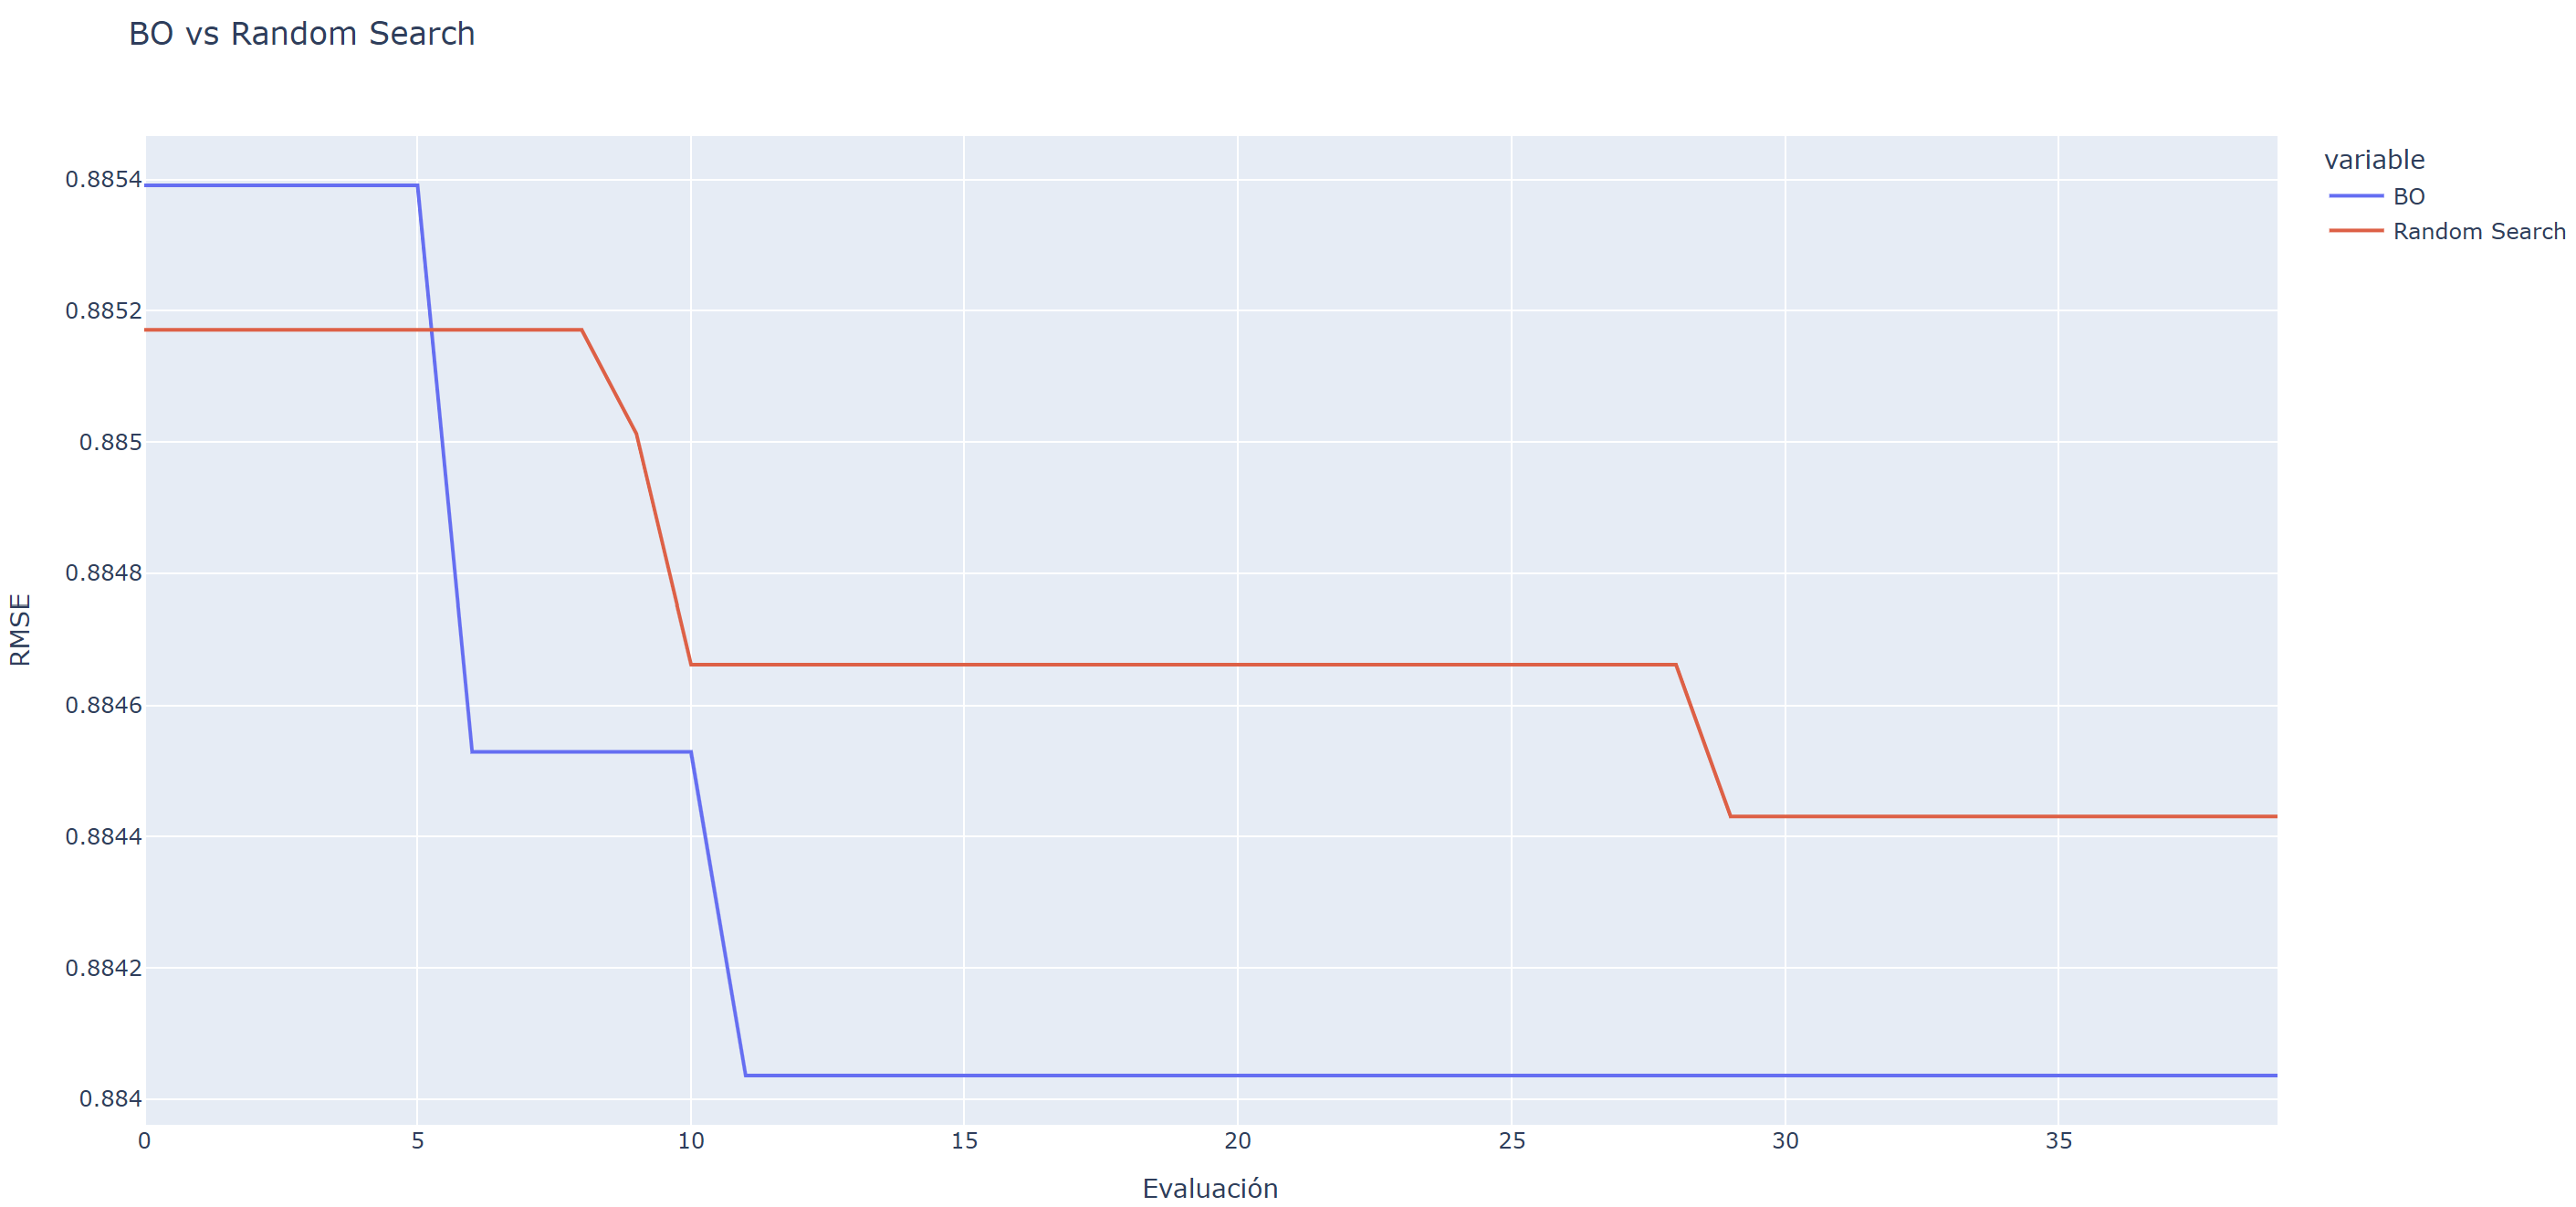
\includegraphics[width=0.47\textwidth]{fig_bo_vs_random.png}
\caption{Convergencia de Bayesian Optimization frente a Random Search}
\label{fig:bo_vs_random}
\end{figure}

\begin{figure}[H]
\centering
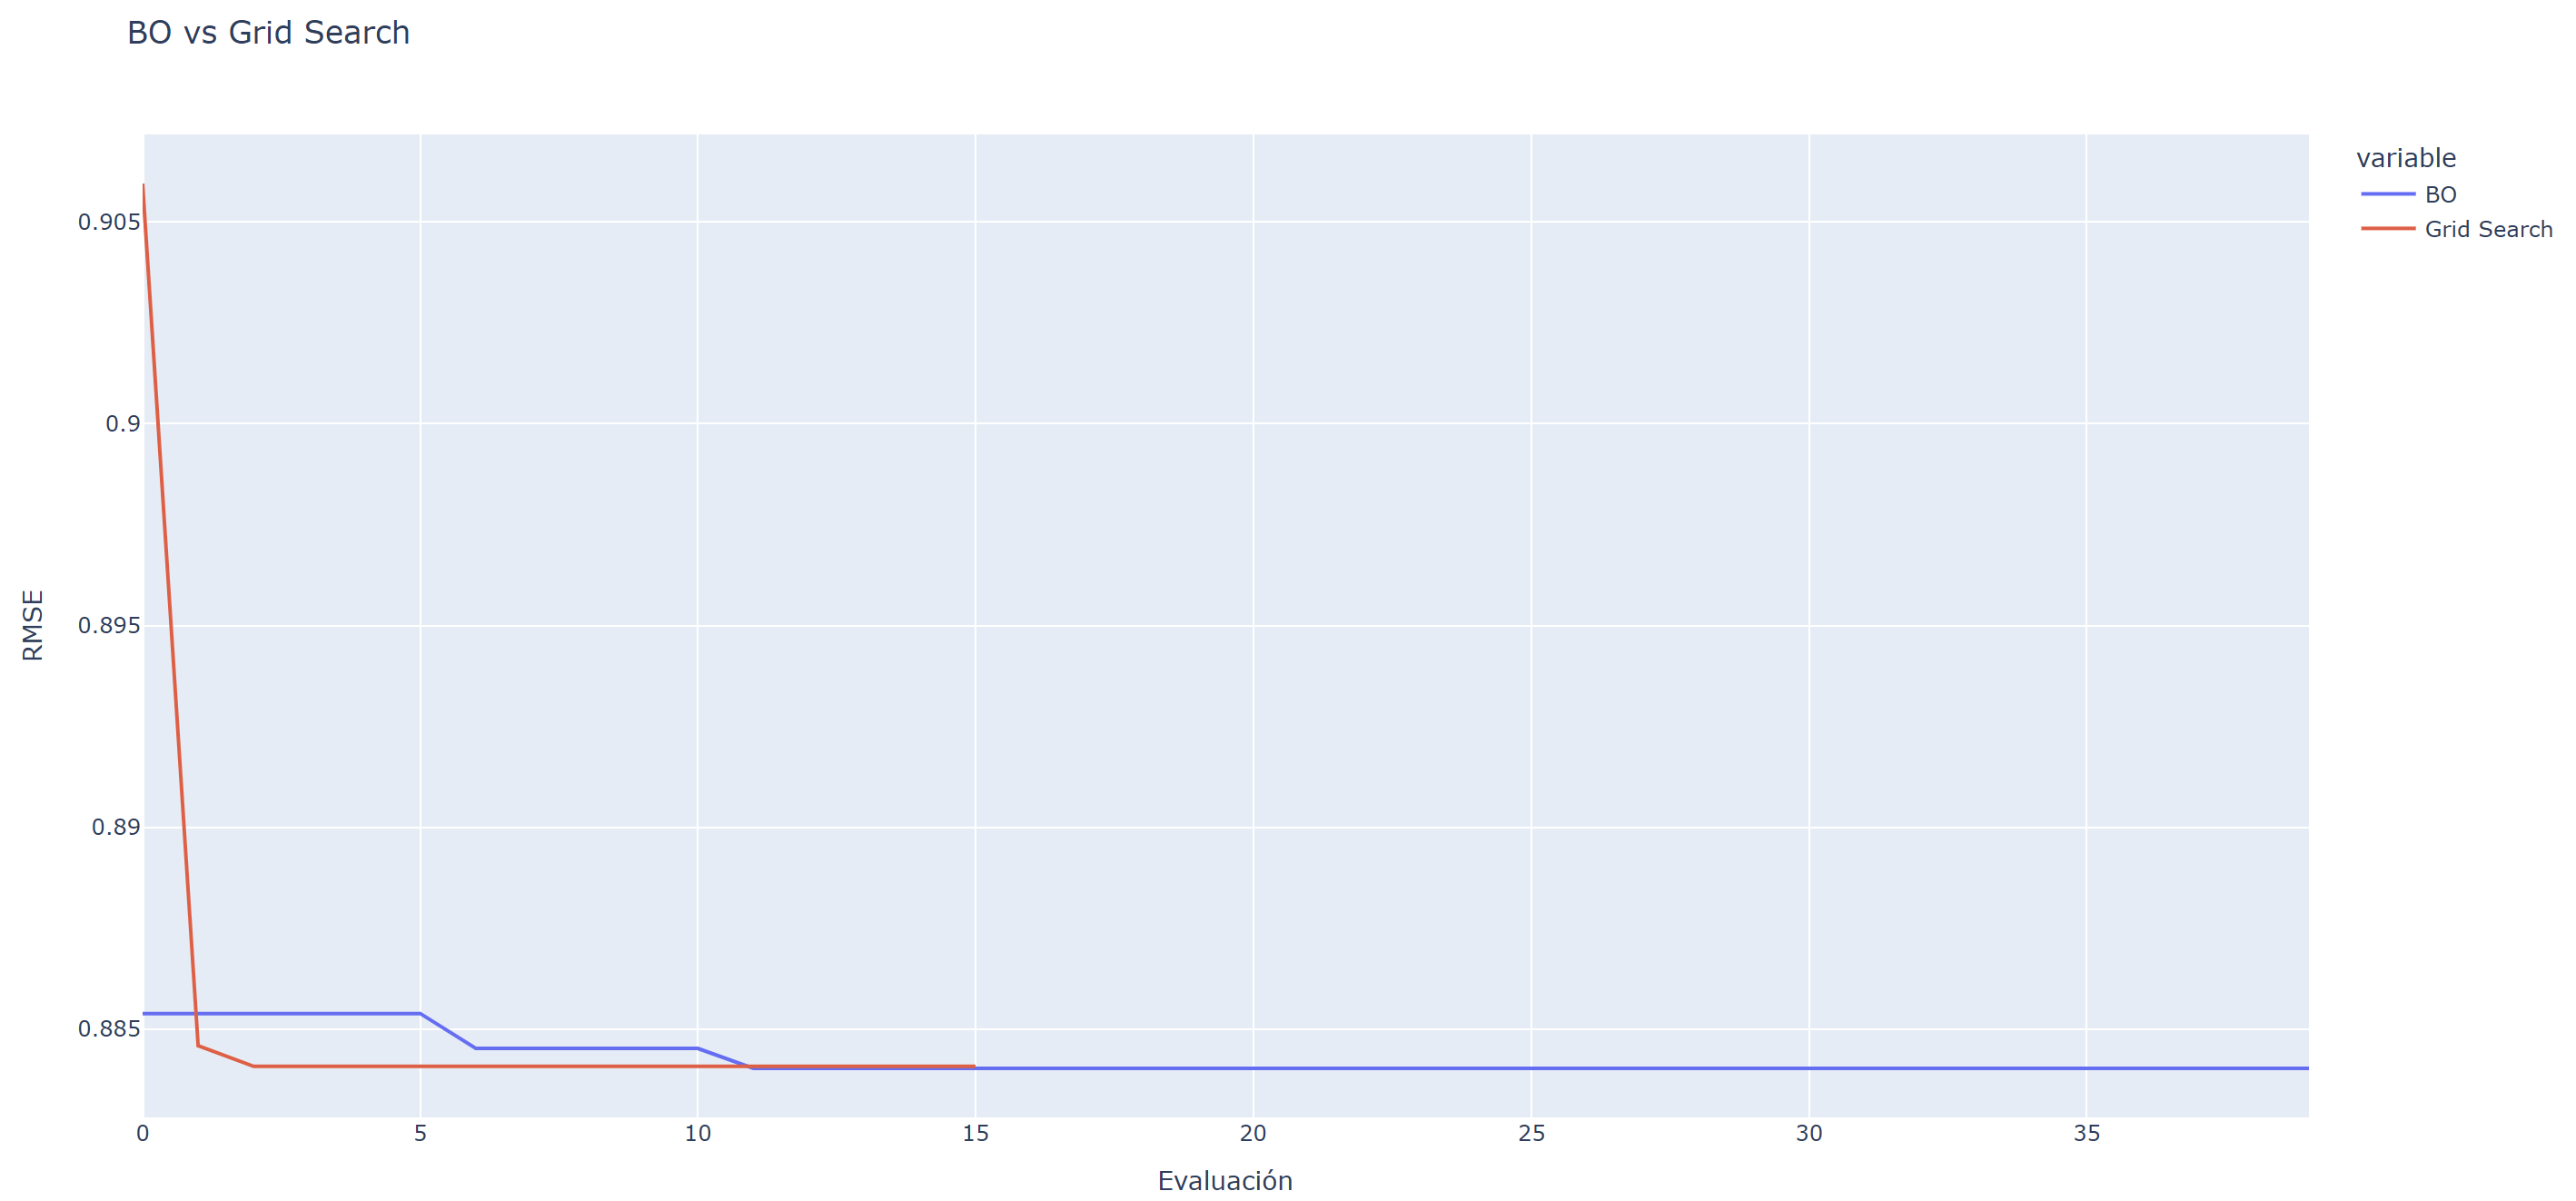
\includegraphics[width=0.47\textwidth]{fig_bo_vs_grid.png}
\caption{Convergencia de Bayesian Optimization frente a Grid Search}
\label{fig:bo_vs_grid}
\end{figure}

Los resultados obtenidos posicionan a la optimización bayesiana como una alternativa robusta para el ajuste de hiperparámetros en sistemas de recomendación. Su capacidad para modelar incertidumbre, incorporar conocimiento previo y encontrar soluciones óptimas con pocas evaluaciones, la convierte en una herramienta adecuada en contextos donde la evaluación de cada configuración implica un costo computacional elevado.

Todo el código fuente desarrollado para esta investigación, incluyendo la implementación de los métodos de optimización y el procesamiento del dataset, se encuentra disponible en un repositorio público mantenido por el autor \citep{kenny2025github}.

\section{Discusión}

\subsection{Ventajas de la optimización bayesiana}

Este estudio mostró que la optimización bayesiana ofrece ventajas concretas sobre métodos como grid search y random search. Aunque las diferencias en el RMSE final fueron pequeñas, el algoritmo bayesiano fue más estable y rápido al explorar el espacio de hiperparámetros, lo que lo hace útil cuando las evaluaciones del modelo consumen mucho tiempo o recursos.

También se observó que se necesitó un menor número de iteraciones para alcanzar configuraciones cercanas al óptimo. Esta eficiencia coincide con lo reportado por \citet{frazier2018tutorial}, quien destaca la utilidad de los modelos sustitutivos en funciones costosas de evaluar. La configuración obtenida ($k = 50$, $\lambda = 0.08$) también guarda similitud con valores reconocidos en trabajos previos como el de \citet{koren2009matrix}, lo que respalda la validez de los resultados.

\subsection{Limitaciones y consideraciones prácticas}

A pesar de sus ventajas, aplicar este tipo de optimización no está libre de retos. Uno de ellos es la sensibilidad a la elección de los puntos iniciales, que puede afectar la estabilidad del proceso, como lo indican \citet{wu2019practical}. Además, seleccionar la función de adquisición más adecuada no siempre es sencillo y puede influir en la calidad del resultado final \citep{brochu2010tutorial}.

Algunos estudios, como el de \citet{wang2020new}, han propuesto formas de reducir estos problemas mediante inicializaciones híbridas. En escenarios como los sistemas de recomendación, donde el tiempo y los recursos son limitados, estas mejoras pueden ser especialmente útiles. Por ello, usar este enfoque requiere un conocimiento claro de sus componentes y una disposición a ajustar sus parámetros según el contexto.

\section{Conclusiones}

Los resultados obtenidos demuestran que la optimización bayesiana es una herramienta eficaz para mejorar modelos de recomendación. Se alcanzó un RMSE competitivo con menos evaluaciones y menor carga computacional frente a técnicas más tradicionales. Esta eficiencia resulta clave en aplicaciones donde se dispone de pocos recursos o tiempo limitado.

Además, los parámetros obtenidos coinciden con los reportados en otros estudios, lo que refuerza la validez del enfoque. A futuro, sería interesante explorar funciones de adquisición más especializadas y aplicar esta técnica a redes neuronales profundas, donde ajustar hiperparámetros de forma eficiente sigue siendo un desafío.

En conjunto, este trabajo respalda el uso de la optimización bayesiana como una alternativa práctica y adaptable en tareas de recomendación.


\section*{Agradecimientos}

Extiendo mi agradecimiento a Fred Torres Cruz por fomentar este tipo de estudios de metodos de optimizacion. Su fundamental contribución fue esencial para esta investigación.

Asimismo, expreso mi gratitud a la comunidad de Optuna. Las herramientas que han proporcionado resultaron ser indispensables para la optimización y el desarrollo de mi estudio. Su soporte fue crucial.
\bibliographystyle{plainnat}
\bibliography{referencias}

\end{document}
